\section{Rastrigin Function}
\label{sec:test_functions:rastrigin}

  The Rastrigin function, first proposed by Rastrigin in 1974\footnote{
    Rastrigin, L. A. (1974). \enquote{Systems of extremal control.} Mir, Moscow.
  }, is a prominent non-convex function utilized as a benchmark for optimization
  algorithms.
  This function is a classic example of non-linear multimodal optimization
  problems, known for their complexity due to the abundance of local minima.

  \begin{definition}[Rastrigin Function]
  \label{def:test_functions:rastrigin}
    The \emph{Rastrigin function}, denoted as \(f:\:\mathbb{R}^n \rightarrow 
    \mathbb{R}\), is formulated as:

    \begin{equation}
    \label{eq:test_functions:rastrigin}
      f(\mathbf{x}) = An + \sum_{i=1}^{n} \left[
        \mathbf{x}_i^2 - A\cos(2\pi \mathbf{x}_i)
      \right]
    \end{equation}
      
    Here, 
    \begin{itemize}
      \item \(n\) is the number of dimensions.
      \item \(\mathbf{x}\) is a vector composed of \(n\) real numbers.
      \item \(A\) is a constant, typically set to 10.
    \end{itemize}

  \end{definition}

  The global minimum of the Rastrigin function is situated at \(\mathbf{x}^* =
  (0, \ldots, 0)\), with \(f(\mathbf{x}^*) = 0\).
  It's particularly challenging due to its numerous local minima, distributed
  regularly throughout the search space. The function is predominantly evaluated
  within the hypercube \(\mathbf{x} \in [-5.12,\, 5.12]^n\).

  Visualizations of the Rastrigin function for \(n = 2\) are presented in
  \vref{fig:test_functions:rastrigin}, showcasing both the contour plot and the
  3D surface plot.

  \begin{figure}[ht!]
    \centering
    \begin{subfigure}[b]{0.45\textwidth}
      \centering
      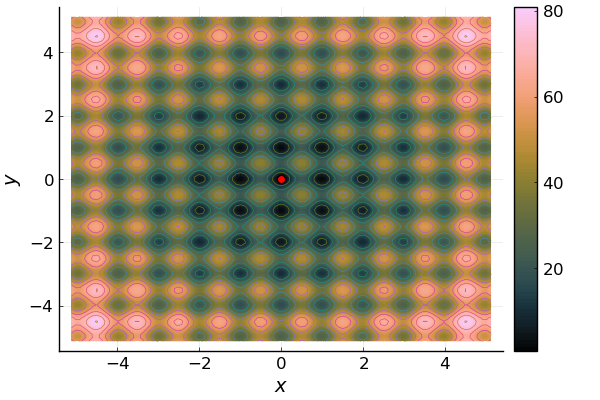
\includegraphics[width=\textwidth]{img/test_functions/rastrigin_contour.png}
      \caption{Contour plot of the Rastrigin Function.}
      \label{fig:test_functions:rastrigin:contour}
    \end{subfigure}
    \hfill
    \begin{subfigure}[b]{0.45\textwidth}
      \centering
      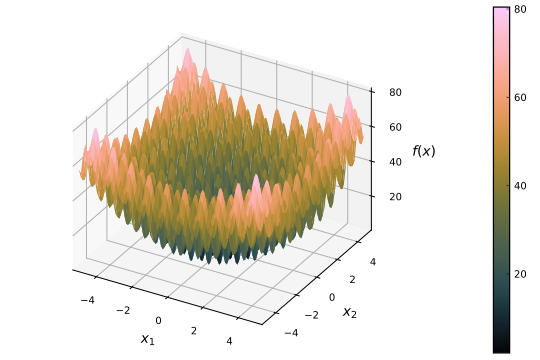
\includegraphics[width=\textwidth]{img/test_functions/rastrigin_surface.png}
      \caption{3D surface plot of the Rastrigin Function.}
      \label{fig:test_functions:rastrigin:surface}
    \end{subfigure}
    \caption{
      Visualizations of the Rastrigin Function for \(n = 2\), with the global
      minimum marked by a red dot.
    }
    \label{fig:test_functions:rastrigin}
  \end{figure}
